\documentclass[12pt,a4paper]{article}
\usepackage[utf8x]{inputenc}
\usepackage{ucs}
\usepackage[german]{babel}
\usepackage{textcomp}
\usepackage{graphicx}
\author{Simon Pruy}



\begin{document}
	\tableofcontents
\section{Impressum}
\section{Hallo erstmal...}
\section{Das Wörterbuch der wahrscheinlich unbekannten Dinge}
	\paragraph{AStA -} \glqq Allgemeiner Studierendenausschuss\grqq . Ist der gewählte Vorsitz des StuPa.
	\paragraph{B.Sc. -}\glqq Bachelor of Science\grqq . Ist der erste Abschluss den ihr als Informatiker bekommen könnt.
	\paragraph{Bachelorordnung -} Das Regelwerk, wie Ihr euren Studienabschluss bekommen könnt. Sollte von jedem Studenten in seinem Studium mindestens einmal gelesen werden!!! Sollten dabei Fragen aufkommen, könnt ihr euch an das Prüfungsamt wenden oder an die Fachschaft.
	\paragraph{Bockenheim, Campus -} Die Großbaustelle, auf der du dich gerade befindest. Außerdem soll hier demnächst ein Kulturcampus entstehen und die Informatik angeblich bis 2017 auf den Riedbergcampus ziehen.
	\paragraph{CP -} \glqq Creditpoints\grqq . Berechnungseinheiten des ECTS(European Credit Point Transfer System), die hochschulübergreifend angerechnet werden können sollten. Dabei gilt: 1 CP $\approx$ 30 Stunden Arbeitsaufwand.
	\paragraph{Dekan -} Text übernehmen!
	\paragraph{Dekanat -} Text übernehmen!
	\paragraph{Direktorium(I-Rat) -} Das Direktorium ist eigentlich der Institutsrat. Anscheinend klang dies zu langweilig, weshalb das Direktorium auch I-Rat genannt wird.
	\paragraph{Direktor, geschäftsführender -} Auch GD genannt, leitet das Direktorium. Außerdem repräsentiert er das Institut nach Außen.
	\paragraph{Direktorat -} Text übernehmen!
	\paragraph{Evaluierung/Evaluation -} Text übernehmen!
	\paragraph{Fachschaftsraum -} Ist der kleine Raum, der an die Studentlounge anschließt. Hier finden Donnerstags ab 16:00 Uhr die Fachschaftstreffen statt.
	\paragraph{Fachschaftstreffen -} Das regelmäßige Treffen der Studierendenvertretung in der Informatik. Es findet Donnerstags ab 16:00 Uhr im Fachschaftsraum statt, wobei am ersten Donnerstag im Monat immer die wichtigen Dinge besprochen werden.
	\paragraph{FBR -} \glqq Fachbereichsrat\grqq. Der FBR ist ein Gremium welches über die zentralen Belange des Fachbereichs 12 entscheidet. Die studentischen Vertreter werden dabei direkt Gewählt.
	\paragraph{Fischerräume -} Die Rechnerräume der Informatik, welche sich hinter dem Magnushörsaal befinden und nur von außen  betretbar sind. Einloggen könnt ihr euch mit eurem RBI-Account.
	\paragraph{FS/FS-Inf -} Text übernehmen, bis auf Seitenangabe!
	\paragraph{HiWis -} Text übernehmen
	\paragraph{Hörsäle -} Die Hörsäle H I - H IV und H 1 - H 16 findet ihr im Hörsaalgebäude.
	\paragraph{HRZ-Account -} Text übernehmen.
	\paragraph{Institutsrat -} Der Institutsrat ist ein Gremium , das die Belange des Institutes Informatik behandelt und teilweise, wo nicht der Fachbereichsrat gefragt ist, entscheidet.
	\paragraph{Kommilitonen -} Sind die Leute links und rechts neben dir.
	\paragraph{Lernzentrum -} Text übernehmen.
	\paragraph{Magnus-Hörsaal -} Ist der einzige Hörsaal, den die Informatik im Gebäude hat.
	\paragraph{Modul -} Text übernehmen.
	\paragraph{M.Sc. -} \glqq Master of Science\grqq . Großer Bruder vom Bachelor.
	\paragraph{Munchkin -} Ein sehr beliebtes Kartenspiel im Fachbereich. 
	\paragraph{Prodekan -} Text übernehmen.
	\paragraph{Prüfungsamt -} Text übernehmen.
	\paragraph{Prüfungsausschuss -} Text übernehmen
	\paragraph{Prüfungsprotokoll-Datenbanken -} Text übernehmen
	\paragraph{QIS-LSF -} Das elektronische Informationssystem der Uni. Hier könnt ihr euch für Prüfungen anmelden, eure Kontaktdaten ändern oder euch den Vorlesungskatalog anschauen. Für das QIS-LSF braucht ihr euren HRZ-Account
	\paragraph{Rekursion -} Rekursion siehe Rekursion!
	\paragraph{RBI -} \glqq Rechner-Betriebsgruppe Informatik\grqq . Die RBI kümmert sich um alles, was mit Elektronik in der Informatik zu tun hat. Über euren RBI-Account, den ihr in der RBI beantragen könnt, habt ihr pro Semester 500 Druckseiten frei und könnt noch weitere Angebote nutzen.
	\paragraph{Skript -} Text übernehmen.
	\paragraph{Statusgruppen -} Text übernehmen.
	\paragraph{Studentlounge -} Text übernehmen.
	\paragraph{Studiendekan -} Text übernehmen.
	\paragraph{Studien-Service-Center -} Befindet sich im PEG-Gebäude auf dem Westend. Hier könnt ihr alle Arten von Anträgen(Teilzeit,etc.) stellen.
	\paragraph{StuPa -} Text übernehmen.
	\paragraph{SWS -} Text übernehmen.
	\paragraph{Tutor -} Als Tutor endet man aus drei verschiedenen Gründen. Ein Grund wäre, dass ihr CP für euer Ergänzungsmodul braucht und euch dadurch entschieden habt Tutor zu werden. Der zweite Grund wäre, dass ihr Geld braucht und für einen Studentlohn von 8,50 Euro arbeiten wollt. Oder aber ihr wollt euer Wissen weiter geben bzw. euer Wissen auffrischen. Eine Mischung aus den drei Gründen tritt auch gelegentlich auf.
	\paragraph{Umzug -} Eine sehr beliebte Sage innerhalb des Fachbereichs 12. Von Generation zu Generation wird weiter verbreitet, dass wir zum Riedberg umziehen werden. Erste historische Erwähnung dieser Sage wurde in den Protokollen der 4. Ratssitzung des Direktorium für Informatik im Jahre 1979 gefunden.
	\paragraph{Wahlen -} Irgendwann werdet ihr ein Brief nach Hause bekommen, womit ihr z.B. den FBR oder das StuPa wählen könnt.
	\paragraph{Westend, Campus -} Der Campus der Geisteswissenschaften. Zu erreichen per Bus mit Linie 36 oder 75, per U-Bahn 1,2,3 oder 8 (Holzhausenstraße) oder falls man Zeit hat auch zu Fuß durch den Palmengarten.
	\paragraph{WiMis -} Text übernehmen
	\section{Euer Studium}
	\subsection{Ein Stundenplan zum Ausfüllen}
	\subsection{BA Informatik}
			\subsubsection{STO}
			\subsubsection{Veranstaltungs- und Prüfungsformen}
	\subsection{Sonstige Studiengänge}
		\subsubsection{MA Info}
		\subsubsection{MA Bioinformatik}
		\subsubsection{MA Wirtschaftsinformatik}
		\subsubsection{Informatik L3}
	
	\subsection{Bachelor-/Masterordnung}

	\subsection{Teilzeitstudium}
	
\newpage
\section{Die Uni}
	\subsection{Wo ist was?}
		\subsubsection{Bockenheim}
			\begin{center}
			\texttt{ It's dangerous to go alone! Take this. }
			
			\fbox{
			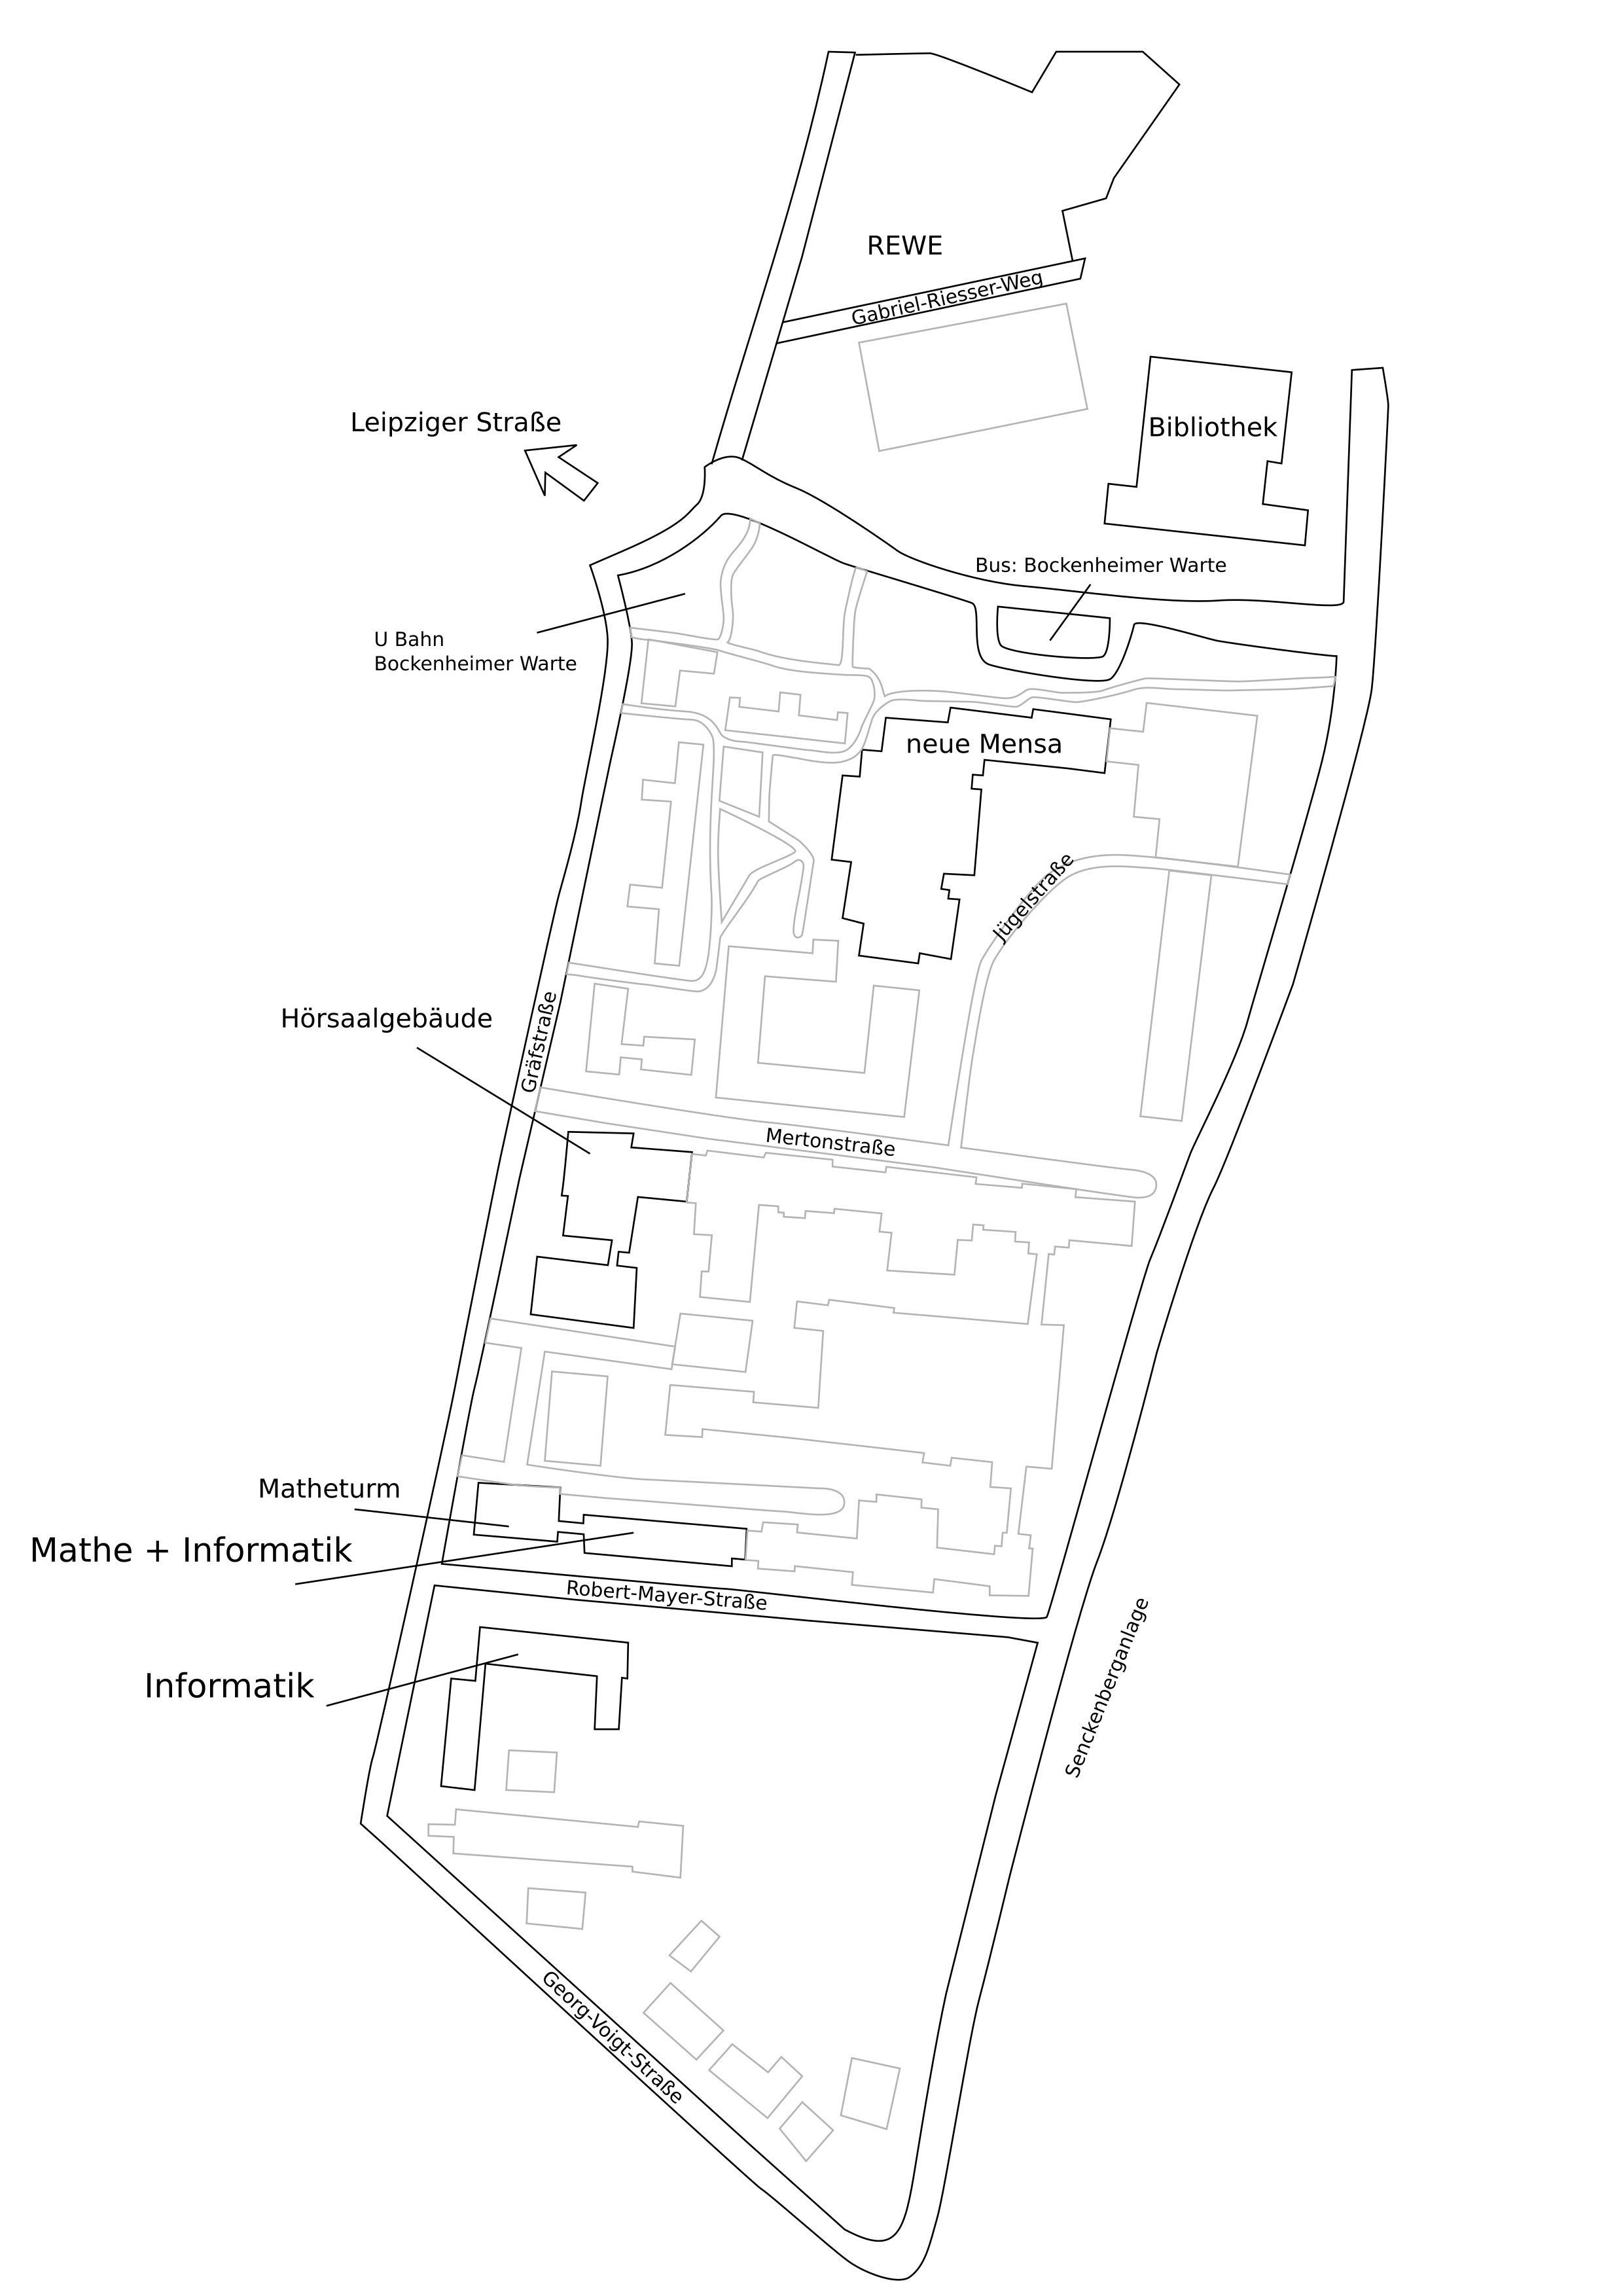
\includegraphics[width=0.9\linewidth]{KarteB}}
			\end{center}
		\pagebreak
			Wichtig für die Vorlesungen und Übungen:\\
			\fbox{
			\begin{tabular}{rrl}
				Hörsäle: & H 1 - H 16  & Teil des Hörsaalgebäudes über dem Cafe.\\
				{} & H I - H VI  & Andere Teil des Hörsaalgebäudes, welcher nicht\\
				{} & {} & über dem Cafe ist.\\
				{} & Magnushörsaal & In der Informatik\\
				{} & {} & {}\\
				Seminarräume: & SR9, SR11 & Informatik EG\\
				{} & 307 & Informatik 3.Stock\\
				{} & NM...& Diese Räume sind in der neuen Mensa\\
				{} & \multicolumn{2}{l}{Alle anderen dreistellingen Zahlen sind im Matheturm}\\
			\end{tabular}}
			\ \\\\ 
			Sonstige Interessante Orte:\\
			\fbox{
				\begin{tabular}{rp{11cm}}
					Cafe Struvelpeter: & Hier gib es Getränke und kaltes Essen. Du findest es im\\
					{} & Hörsaalgebäude.\\
					Cafeteria: & Verkauft warme Gerichte und gehört zum Studentwerk.  \\
					{} & Ihr findet die Cafeteria in der neuen Mensa.\\
					Leipziger Straße: & Falls ihr aus gegebenen Anlässen keine Lust mehr auf Mensa essen habt, dann gibt es hier alles was das Herz begehrt(Nicht nur Essen).
				\end{tabular}
			}
		
		\subsubsection{Westend}
			Das Westend ist für euer Studium erst interessant, wenn ihr ein Anwendungsfach der Geisteswissenschaften gewählt habt oder ihr Fragen oder Probleme mit dem HRZ oder der Uni habt. Außerdem ist das Westend ein perfekter Ort für eine Studentensafari. Nirgendwo sonst gibt es einen Lebensraum, wo die Reviere so unterschiedlicher Studenten aufeinander treffen. \\
		
		\subsubsection{Riedberg}
			Genauso wie das Westend, ist der Riedberg erst mit der Wahl eines Anwendungsfaches interessant. Bis auf der Tatsache, dass wir uns von Anfang an dort wohlfühlen.
		\subsubsection{Niederrad und Ginnheim}
			Orte, wo die meisten von uns nie sein werden. In Ginnheim befinden sich die Unisportanlagen und in Niederrad die Medizin.
	
		
	\subsection{QIS/LSF und dessen Funktion}
	\subsection{Hilfsmittel für den Unialltag}
		\subsubsection{Goethe-Card + Semesterticket}
		\subsubsection{Internet}
		\subsubsection{Softwarelizenzen}
		\subsubsection{Bücherreien}
	\subsection{Aufbau der Unipolitik}
\section{Die Informatik}
	\subsection{Robocup-AG}
\section{Die Fachschaft}
	\subsection{Wer sind wir?}
		\glqq\textit{ Wir befinden uns im Jahre 2015 n.Chr. Die ganze Informatik ist von der Faulheit besetzt... Die ganze Informatik? Nein! Ein von unbeugsamen Freiwilligen bevölkerter Raum hört nicht auf, dem Eindringling  Widerstand zu leisten.} \grqq \\
		Spaß beiseite. Wir sind die aktive Fachschaft der Informatik. Aktiv, weil alle Studenten Teil der Fachschaft sind. \\
		Grundsätzlich kann man aber über uns sagen, dass wir ein versprengter Haufen von verrückten, abgedrehten Nerds, Geeks und anderer Lebensformen in den Augen von Außenstehenden sind, dies aber teilweise auf Vorurteilen  
	beruht. Welche davon stimmen und welche nicht, dürft ihr gerne selber herausfinden. Wir bezeichnen uns aber gerne als normal. 	
	\subsection{Was machen wir}
		Das grundlegende Vorurteil gegenüber eine Informatik-Fachschaft besteht darin, dass wir ständig am Trinken und am Rollenspiele spielen sind. \\
		Damit die Wahrheit ans Licht kommt, müssen wir aber sagen, ja das stimmt teilweise (welcher Teil nun stimmt, bleibt wieder euch überlassen). Aber das ist nur ein kleiner Teil unserer Arbeit.\\
		Der andere große Teil betrifft hauptsächlich den Universitätsalltag.\\ Viel Zeit verbringen wir z.B. mit Gremienarbeit, wo wir derzeit die studentischen Vertreter stellen. Zu diesen Gremien zählen derzeit:
		\begin{itemize}
			\item I-Rat
			\item FBR
			\item Lust-Ausschuss
			\item Prüfungsausschüsse
			\item QSL-Mittelausschuss
			\item FSR
			\item FSK	
		\end{itemize}
		Zu unseren weiteren Aufgaben zählt auch, dass wir anderen Studenten helfen. Dies kann auf unterschiedlichste Weise passieren:
		\begin{itemize}
			\item Bei Fragen zu organisatorischen Themen können wir selber Antworten geben oder auf Personen verweisen, die euch da besser weiter helfen können.
			\item Falls ihr berechtigte Kritik an Vorlesungen und/oder Übungen nicht selbst äußern wollt oder sie ignoriert wird, sind wir dafür da, diese Kritik an die verantwortliche Person weiter zu tragen, wozu uns mehr Möglichkeiten zur Verfügung stehen.
			\item Wir organisieren die OE für Erstsemestler, damit ihr in der ersten Woche nicht vor lauter ungewohnten Sachen erschlagen werdet.
			\item Wir erstellen dieses Heft, damit ihr wichtige Themen nachschlagen könnt.
			\item Wir organisieren Sommerfest und Weihnachtsfeier!
		\end{itemize}
		
	\subsection{Du willst zu uns?}
		\glqq Wir grillen gerade und haben ein wenig zu trinken da. Willst du nicht zu uns stoßen?\grqq { }Bei vielen Fachschaftlern hat diese Masche schon funktioniert. Doch gerüchteweise gibt es unter den Studenten auch immer ein paar ''Rationalisten'' die ''Argumente'' brauchen. Und weil ''Wir sind cool!'' nicht immer ausreicht, sind hier ein paar Kommentare von und über uns:
		\begin{itemize}
			\item Wir sind cool!
			\item Social Engeneering lernen, wo besser als an der Uni?
			\item Die Gerüchteküche sind wir.
			\item Form die Uni nach eurem Bild.
			\item Lern die Professoren kennen.
			\item Mach die Uni zu deinem Zuhause and der Uni.
			\item Lern die Studenten kennen, die das dir dein 2h Problem in 2min lösen.
			\item Werde Student, der die 2h Probleme in 2min löst.
			\item CP für Gremienarbeit.
			\item Das Direktorat fragt dich.
			\item Entscheide für wen Ausnahmen gemacht werden.
			\item Firmenpolitik begegnet dir überall. Lerne die Kunst an der Uni.
			\item Bekomme Schlüssel
			\item Fachschaftsfeiern
		\end{itemize}

	
	
\end{document}